\documentclass[11pt]{article}
\usepackage[a4paper,margin=25mm]{geometry}
\usepackage[T1]{fontenc}
\usepackage{lmodern,microtype,amsmath,amssymb,amsthm,mathtools}
\usepackage{booktabs,longtable,tabularx,array,enumitem,xcolor,graphicx}
\usepackage{fancyhdr,hyperref,xurl,listings}
\definecolor{ink}{HTML}{15354B}
\definecolor{accent}{HTML}{176B87}
\definecolor{soft}{HTML}{EDF4F7}
\hypersetup{colorlinks=true,linkcolor=accent,citecolor=accent,urlcolor=accent,
 pdftitle={Exact Quotient Kernels for Unknot Recognition},
 pdfauthor={ProveIt research continuation}}
\pagestyle{fancy}\fancyhf{}
\fancyhead[L]{\small\color{ink}Exact quotient kernels for unknot recognition}
\fancyhead[R]{\small ProveIt / 2026-10-08}
\fancyfoot[C]{\thepage}
\setlength{\headheight}{14pt}
\setlength{\emergencystretch}{2em}
\setlist{itemsep=3pt,topsep=5pt}
\newtheorem{theorem}{Theorem}[section]
\newtheorem{proposition}[theorem]{Proposition}
\newtheorem{lemma}[theorem]{Lemma}
\newtheorem{corollary}[theorem]{Corollary}
\theoremstyle{definition}
\newtheorem{definition}[theorem]{Definition}
\newtheorem{example}[theorem]{Example}
\newtheorem{remark}[theorem]{Remark}
\newcommand{\F}{\mathbb F_2}
\newcommand{\End}{\operatorname{End}}
\newcommand{\Span}{\operatorname{span}}
\newcommand{\rank}{\operatorname{rank}}
\newcommand{\im}{\operatorname{im}}
\newcommand{\id}{\operatorname{id}}
\newcommand{\poly}{\operatorname{poly}}
\newcommand{\code}[1]{\texttt{#1}}
\lstset{basicstyle=\ttfamily\footnotesize,breaklines=true,
 backgroundcolor=\color{soft},frame=single,rulecolor=\color{soft},
 columns=fullflexible,keepspaces=true,showstringspaces=false,upquote=true}

\begin{document}
\begin{titlepage}
\color{ink}
\vspace*{13mm}
{\large\sffamily PROVEIT RESEARCH CONTINUATION\par}
\vspace{12mm}
{\huge\bfseries Exact Quotient Kernels\\[3mm]for Unknot Recognition\par}
\vspace{8mm}
{\Large Sharp interval mergers, scalar gauges,\\and simultaneous cyclic overlap search\par}
\vspace{12mm}
{\large 8 October 2026\par}
\vspace{12mm}
\noindent\begin{minipage}{0.94\textwidth}
\textbf{Research status.} This report supplies exact local algorithms, proofs,
native implementations, independent correctness comparisons and measured
performance evidence. It does not establish a general quasi-polynomial
unknot-recognition bound. The strongest unconditional complexity improvements
apply to explicitly specified subproblems; the complete recognizer retains
its previous general complexity status.
\end{minipage}
\vfill
\noindent\textbf{Pinned baseline}\par
\small\path{VladimirReshetnikov/ProveIt}\par
\path{58ee11a97d5fd7f21647c57eefaf3ecc007931d6}\par
\path{Topology/UnknotRecognition/fast}\par
\vspace{5mm}
\noindent The accompanying archive contains the maintained source overlay,
an integration patch, the full article source, reproducible experiments,
raw results, tests, provenance and checksums.
\end{titlepage}

\begin{abstract}
Three sources of repeated work remain visible in the maintained unknot
recognizer and its geometric research components: periodic interval regions
are processed separately, scalar endomorphism solvers expand dependent
morphism coefficients, and explicit group simplification searches the same
relator collection once for each donor. We develop exact quotients for these
three situations. First, a Fine--Wilf argument gives the necessary and
sufficient overlap threshold $p+q-\gcd(p,q)$ for replacing two periodic
interval relations by their gcd relation. An independent
Agol--Hass--Thurston implementation uses this rule, and a native adapter
counts components, boundary curves and orientability directly from binary
normal coordinates in a validated finite torus-boundary triangulation.
Second, typed differential blocks are factored through their actual
coefficient spans. Invertible coefficient matrices then eliminate redundant
endomorphism unknowns along a forest without identifying distinct chain
objects. The complete commutant is reconstructed in canonical coordinates,
so bounded candidate selection is preserved. Third, a shared index solves
the explicit all-pairs cyclic relator-overlap problem; a bounded incumbent
search exploits the elementary donor-length bound before invoking that
index. The report distinguishes proof, implementation, observed activation
and the missing global representation-size bounds throughout. Classical
ingredients are attributed explicitly; no priority claim is made for the
underlying orbit-counting, periodicity, suffix-automaton or linear-algebra
theorems.
\end{abstract}
\tableofcontents
\newpage

\section{The baseline and the research objective}

The requested target is an exact unknot recognizer with running time
$n^{O(\log n)}$, where $n$ is the size of an ordinary knot diagram. The
repository already contains a substantial exact pipeline: diagram
simplification, structural certificates, polynomial and group-theoretic
filters, specialized braid routes, and scanning Khovanov backends. It also
contains separate research kernels for compressed geometric operations.
Our baseline is the Git commit printed on the title page, committed on
8 October 2026 at 19:17:11 UTC. All integration comparisons refer to that
snapshot; reports created against earlier snapshots are not silently treated
as the incumbent implementation.

The present work concerns three concrete computational tasks. The first is
geometric connectivity for a normal surface whose coordinate sum may be
exponential in the triangulation size. The second is the exact scalar
commutant of a typed differential, which is used to discover direct-sum
splittings. The third is maximum guaranteed shortening by a single cyclic
relator replacement. Each task has a finite, independently checkable
specification. Improvements to them can be verified without assuming the
desired global recognition theorem.

Lackenby's 2026 hierarchy paper gives new incompressibility and unknot
algorithms, while explicitly leaving a running-time specification for
several operations incomplete. Its Proposition 9.1 bounds repeated steps
by $L(g+1)^L$ in terms of hierarchy length and pattern complexity. The
refined construction supplies a linear bound on hierarchy length in the
initial $q$-complexity. These are significant structural facts, but neither
is by itself a quasi-polynomial bound for the encoded implementation
\cite{lackenby2026}. The 2021 lecture announces the intended accelerated
framework \cite{lackenbytalk}. We use these as motivation and as a precise
list of remaining obligations, rather than interpreting efficient local
arithmetic as a proof of the complete algorithm.

\subsection{What the report contributes}

\begin{enumerate}
\item An exact two-period merger criterion, with a necessity argument and
an explicit family showing a linear reduction in the number of orbit
algorithm cycles. This is a sharpened application of the classical
Fine--Wilf theorem within the AHT algorithm.
\item A native, coordinate-compressed topology query for arbitrary
admissible normal vectors in its stated class of finite triangulations.
It supports disconnected and one-sided surfaces and does not require an
extreme-ray witness.
\item Exact coefficient-span and forest substitutions in the scalar
endomorphism equations, including reconstruction of the entire original
solution space and preservation of its canonical basis.
\item A simultaneous index and a bounded adaptive policy for explicit
cyclic relator overlaps, replacing an all-donor repeated scan with a
near-linear local query in the specified computational model.
\item Reproducible comparisons against the pinned code and independent
small oracles, together with corrections, negative measurements and a
concrete research agenda.
\end{enumerate}

The full general recognition bound remains unproved. In particular, this
work does not bound intermediate Khovanov multiplicities, the total length
of explicit group presentations, the number of relator moves, the complete
encoding of a cut manifold, or the number of hierarchy repairs. Those
quantities cannot be omitted from the complexity accounting.

\section{Representations and cost parameters}

It is useful to distinguish an expanded object from its stored description.
The relevant parameters are summarized below. A parameter belonging to one
subproblem is never substituted for diagram size without a separate proof.

\begin{center}\small
\begin{tabularx}{\textwidth}{@{}lX@{}}
\toprule
Parameter & Meaning\\\midrule
$n$ & Number of crossings, together with the ordinary diagram encoding.\\
$t,W$ & Tetrahedron count and sum of the seven normal coordinates per tetrahedron.\\
$N,k$ & Number of integer points and number of interval pairings in an orbit query.\\
$b$ & Bit length $\lceil\log_2(N+1)\rceil$ of interval endpoints.\\
$s_v$ & Dimension of one scalar type in a differential component.\\
$V$ & Number $\sum_v s_v^2$ of original scalar endomorphism variables.\\
$\rho_{uv}$ & Dimension of the span of coefficient values in differential block $D_{vu}$.\\
$V_F$ & Number of remaining matrix variables after the chosen invertible forest.\\
$m,\ell$ & Number of nonempty explicit relators and their total expanded letter length.\\
\bottomrule
\end{tabularx}
\end{center}

An interval pairing stores a constant number of $b$-bit integers. A normal
vector stores $7t$ integers; $W$ may be exponentially larger than that input.
The new orbit algorithms operate on endpoints, never on a list of $N$
points. Conversely, the new relator index takes explicit words. It does not
turn a straight-line grammar of exponentially long words into a polynomial
explicit string. The existing compressed-word route remains a different
algorithm with its own contracts.

For binary linear algebra we count bit operations conservatively. A Python
integer containing a packed coefficient is not a unit-cost scalar of
unlimited size. Its XOR, shift and bit-count costs depend on its length.
For the string index, dictionary-operation bounds and bit-complexity bounds
are distinguished. These distinctions matter when comparing an apparent
constant-size formula with the actual stored input.

\section{An exact merger theorem for periodic interval relations}
\label{sec:merger}

Let $R=[a,z]\cap\mathbb Z$ and let $p>0$. A periodic pairing of period $p$
identifies $x$ and $x+p$ whenever both lie in $R$. In the implementation it
is represented by $[a,z-p]\to[a+p,z]$. We call it periodic only when its
domain width is at least $p$, equivalently $|R|\ge2p$. Its orbits in $R$
are exactly the $p$ residue classes modulo $p$.

Suppose two such relations have supports $R_1,R_2$, periods $p,q$, and
overlap of size $h=|R_1\cap R_2|$. Write $d=\gcd(p,q)$. The original AHT
periodic merger uses the sufficient condition $h\ge p+q$
\cite{aht}. The following criterion removes the unnecessary $d$ points.

\begin{theorem}[Exact two-period merger]
\label{thm:sharpmerge}
For two periodic pairings as above, their generated equivalence relation
on $R_1\cup R_2$ is the residue relation modulo $d$ if and only if
\[
                         h\ge p+q-d.
\]
Thus, under this condition, they may be replaced by a single periodic
pairing of period $d$ on the union. The equivalence remains valid in the
presence of any additional pairings.
\end{theorem}

\begin{proof}
Every old identification preserves residue modulo $d$, so it cannot
identify points of different $d$-classes. Color each point of the
intersection by its orbit under the two old relations. This finite color
sequence has periods $p$ and $q$: two intersection points separated by
either period already lie in one of the periodic supports. If
$h\ge p+q-d$, the Fine--Wilf theorem \cite{finewilf} says that the color
sequence has period $d$. Moreover $p+q-d\ge\max(p,q)$, so the intersection
contains a representative of every residue class of both original
supports. Every point outside the intersection is therefore linked to an
intersection point of the same $d$-class. This proves sufficiency.

For necessity, contract the first support to its $p$ residue classes and
the second to its $q$ residue classes. Before identifying their common
points there are $p+q$ vertices. Each of the $h$ common points contributes
one edge between the corresponding two residue vertices, allowing parallel edges but no further identifications. A graph with
$p+q$ vertices and $h$ edges has at least $p+q-h$ connected components.
If $h<p+q-d$, this exceeds $d$. The residue relation modulo $d$ has exactly
$d$ classes on the union, so replacement would change the equivalence
relation. Finally, equality of the two generated relations is preserved
when a common collection of additional generators is adjoined.
\end{proof}

The necessity statement concerns these two generators alone. Other
pairings can create extra connections and can justify mergers below this
threshold. The implementation never infers that a failed two-generator
test proves global disconnectedness.

\begin{example}[The endpoint matters]
The pairings $[0,3]\to[2,5]$ and $[2,4]\to[5,7]$ have periods $2,3$
and an overlap of four points. They generate a connected relation and
can be replaced by a period-one relation. The original five-point
condition misses this merger. Moving the second support one point to
the right leaves only three common points and produces two orbits;
the period-one replacement would then be incorrect.
\end{example}

\subsection{A family with a linear reduction in orbit cycles}

\begin{proposition}[Adjacent periodic blocks]
\label{prop:chain}
For $r\ge1$ and $p\ge1$, consider $r$ pairings
\[
 [ip,(i+1)p-1]\longrightarrow[(i+1)p,(i+2)p-1],
 \qquad 0\le i<r,
\]
on $N=(r+1)p$ points. Both orbit algorithms return $p$. With the stated
maximal-transmission and suffix-truncation policy, the original AHT merger
requires $r+1$ cycles, while the sharp merger requires two.
\end{proposition}

\begin{proof}
Each pairing joins equal positions in two consecutive blocks. Therefore
the $p$ positions within a block label the complete orbits. Neighboring
supports overlap in $p$ points, below the old $2p$ threshold, and
nonneighbors overlap in fewer points. The rightmost pairing is the only
one meeting the last block. No other range is contained in its range,
so one suffix truncation deletes this block and this pairing. Induction
leaves one block after $r$ cycles; a final static contraction counts its
$p$ points.

Under Theorem~\ref{thm:sharpmerge}, neighboring period-$p$ supports meet
the exact threshold $p$. Repeated merging combines all pairings in the
first cycle. The resulting single pairing sends $[0,rp-1]$ to
$[p,(r+1)p-1]$. Suffix truncation removes its entire range, leaving
$[0,p-1]$; the second cycle counts these $p$ static points.
\end{proof}

This is a cycle-count theorem for an explicit interval family, not a
family of knot diagrams. The straightforward implementation additionally
spends time scanning candidate pairs. The benchmark records both cycles
and candidate tests rather than using cycle count as a proxy for elapsed
time.

\section{Native orbit counting and signed components}

The implementation \path{fastunknot/interval_orbits.py} follows the
classical unweighted AHT reduction. Identity relations are removed,
uncovered intervals are counted and contracted, overlapping reflections
are trimmed, valid periodic pairs are merged, other ranges are transmitted
through a maximal rightmost pairing, and its exclusive suffix is removed.
Powers of a translation are evaluated by integer division, avoiding an
iteration per translated point. These transformations and the polynomial
termination theorem are classical \cite{aht}; the sharp merger is the
specific change analyzed in Section~\ref{sec:merger}.

\subsection{Why the stronger rule retains polynomial termination}

The AHT analysis uses a multiplicative quantity of the form
$X=4^k\prod_i w_i$, where $w_i$ are pairing widths. It is not necessary
for every individual cycle to halve $X$. The classical proof bounds the
number of cycles between sufficient reductions of this quantity.

For a sharp merger, the two old widths are $w_1,w_2$ and the new width is
\[
 w'=w_1+w_2+p+q-h-d\le w_1+w_2\le2w_1w_2.
\]
Thus $k$ decreases by one and the contribution to $X$ drops by at least
a factor of two. A state with no sharp merger also has no original AHT
merger, so the hypotheses needed by the remaining classical progress
argument still hold. The strengthened reduction therefore keeps a
polynomial bound in $k$ and $\log(N+1)$. The implementation uses simple
lists and pair scans; it is not claimed to attain the smallest possible
polynomial exponent.

The stored number of pairings never increases in a count query. All
endpoints remain within the original interval. Arithmetic has bounded
bit length, and the largest translation powers are handled in one division.
The number of represented points is allowed to be vastly larger than
memory because it is never used as an iteration bound.

\subsection{Signed gluing and orientation consistency}

An order-reversing map of a sheet interval need not reverse surface
orientation. These are distinct pieces of data. For a pairing $g_i$,
let $\epsilon_i\in\F$ be a separately specified parity. A component is
consistent when the parity sum around every closed walk is zero.

\begin{proposition}[Two-sheeted count]
\label{prop:signed}
Let $C$ be the number of original orbits and $\widehat C$ the number of
orbits of
\[
 (x,e)\sim(g_i(x),e+\epsilon_i),\qquad e\in\F.
\]
Then the numbers of consistent and inconsistent components are
\[
                    C_{+}=\widehat C-C,\qquad
                    C_{-}=2C-\widehat C.
\]
The lifted system is represented by $2k$ interval pairings on $2N$
points, so both counts have polynomial bit complexity in the original
description length.
\end{proposition}

\begin{proof}
Fix a base component and one lift of a chosen point. If all closed
walks have parity zero, continuation of this lift determines one sheet
at every point; the two choices of initial sheet give two disjoint lifted
components. If some closed walk has odd parity, the two initial sheets
are connected and the lift is connected. Thus
$C=C_++C_-$ and $\widehat C=2C_++C_-$. Solving the two equations gives
the formulas. Two consecutive blocks of $N$ integers encode the sheets;
each old interval pairing gives one map from each sheet to its prescribed
target sheet.
\end{proof}

\begin{proposition}[Point membership without extraction]
Two supplied points $x,y$ belong to the same orbit if and only if
adjoining the singleton relation $x\sim y$ leaves the number of orbits
unchanged. If they were in distinct orbits, this addition reduces the
number by exactly one.
\end{proposition}

This gives an exact membership query using two counts. It does not
extract the normal coordinates or attachment data of a chosen component.
Weighted AHT, which is a classical extension, remains a separate
implementation task.

\section{Binary normal-surface topology in a supplied triangulation}
\label{sec:normal}

The new adapter accepts a nonempty finite tetrahedral face-pairing
description of a connected compact orientable 3-manifold with exactly
one torus boundary. Its native validator checks reciprocal face gluings,
edge orientations, edge links, vertex links, orientability, connectedness
and boundary topology. This validator is adapted, with attribution, from
the earlier report 36 normal-disc certificate. The current extension
accepts every nonnegative admissible normal vector in that ambient class;
it does not impose primitivity or an extreme-ray rank condition.

Normal coordinates in each tetrahedron are
\[
 (T_0,T_1,T_2,T_3,Q_{01|23},Q_{02|13},Q_{03|12}).
\]
All matching equations and the condition of at most one nonzero
quadrilateral type per tetrahedron are checked using exact integers.
Hexadecimal integer input is supported. The empty surface is represented
by the zero vector and has no components.

\subsection{The arc-pairing construction}

Give each global triangulation edge a fixed direction. A parity
union-find transports local edge directions through face gluings; using
vertex labels alone would be wrong in a one-vertex triangulation. If a
global edge meets the normal surface $w_e$ times, allocate an interval
of $w_e$ points ordered along this direction. The disjoint union of
these intervals has
\[
                            N=\sum_e w_e
\]
points. Each tetrahedral normal disc meets at most four edges, so
$N\le4W$.

In a triangular face opposite vertex $f$, the normal arcs cutting off
a vertex $v$ occur with multiplicity
\[
                       a_{fv}=T_v+Q_{fv},
\]
where $Q_{fv}$ denotes the quadrilateral type disjoint from the edge
$\{f,v\}$. These arcs join the $a_{fv}$ endpoints nearest $v$ on its
two incident face edges, in their common order from $v$. Consequently
the whole parallel family is one interval isometry, possibly reversing
the globally chosen edge orders. One copy of every glued face and every
boundary face suffices. There are at most three pairings per face,
and therefore $O(t)$ pairings overall.

\begin{theorem}[Normal-surface topology query]
\label{thm:normal}
For an admissible normal surface $S$ in the supported triangulation
class, the adapter and unbounded orbit kernel compute the following in
time polynomial in $t$ and $\log(W+1)$:
\begin{enumerate}
\item the number of components of $S$;
\item the numbers of orientable and nonorientable components;
\item the number of boundary curves of $S$;
\item the total Euler characteristic of $S$.
\end{enumerate}
When $S$ is connected these data determine its genus or crosscap number.
No normal disc or edge intersection point is expanded.
\end{theorem}

\begin{proof}
The constructed graph is the one-skeleton of the normal cell structure,
with each parallel arc family encoded as an interval pairing. Every
normal disc is attached along a connected polygonal boundary. Attaching
such discs does not merge different components of the one-skeleton.
Conversely, every point of a disc can be joined inside the disc to its
boundary. Thus graph components and surface components are identical.
This is the classical normal-surface reduction to AHT connectivity
\cite{aht}, now made explicit in the native coordinate adapter.

For the boundary count, retain only boundary faces and boundary edge
intervals. Every vertex of this normal boundary graph has degree two,
so its components are precisely the boundary circles. Interior edge
points must be removed from this query; leaving them as isolated
vertices would falsely increase the boundary count.

The normal surface with coordinates $2S$ is the horizontal boundary
of the normal interval bundle of $S$. In an orientable ambient
3-manifold this is the orientation double cover. If its component
count is $C_2$, then $C_2-C$ original components are orientable and
$2C-C_2$ are nonorientable, by the same covering argument as
Proposition~\ref{prop:signed}. The vertical annuli over $\partial S$
are not included in this statement.

Finally, the cell counts are obtained arithmetically: vertices are
$\sum_e w_e$, edges are the sums of normal-arc multiplicities over
each face taken once, and faces are the $W$ discs. Hence
\[
             \chi(S)=\sum_e w_e-
                 \sum_{\text{global faces }F}\#(S\cap F)+W.
\]
For a connected orientable surface of genus $g$ with $b$ boundary
curves, $2g=2-b-\chi(S)$; for a connected nonorientable surface the
crosscap number is $2-b-\chi(S)$. Construction and validation use
$O(t)$ combinatorial records and binary arithmetic. The three orbit
systems have $O(t)$ pairings and endpoint lengths
$O(1+\log(W+1))$, completing the complexity claim.
\end{proof}

\subsection{Compressing discs and the correspondence still needed}

If $S$ is connected, has Euler characteristic one and one boundary
curve, it is a disc. On a torus, an embedded simple closed curve is
essential exactly when its mod-two homology class is nonzero. The
adapter computes the dual boundary cocycle by taking $w_e\bmod2$ on
each boundary edge. It tests whether this cocycle is a vertex
coboundary by parity propagation. A nonzero class therefore proves
that the disc compresses the supplied boundary torus.

The output is a relative statement about this triangulation. It is
not a PD-level unknot certificate: the triangulation-to-knot
correspondence is not established by this module. Nor does the module
search for the normal vector. A successful topology calculation must
not be substituted for a missing exterior-construction certificate.

\subsection{Large multiplicities and one-sided surfaces}

For a two-sided normal disc $D$, the vector $aD$ represents $a$
parallel discs. The output component count may therefore be a
500-bit integer while the description uses only a fixed number of
coordinates. For a one-sided normal M\"obius band $M$, the vector
$aM$ has $\lfloor a/2\rfloor$ annuli and, when $a$ is odd, one
M\"obius band. In particular,
\[
 C(aM)=\lceil a/2\rceil,\quad
 C_+(aM)=\lfloor a/2\rfloor,\quad
 C_-(aM)=a\bmod2.
\]
These formulas are independent checks of the doubling calculation.
The tests include multiplicities exceeding $2^{500}$.

The inherited Fibonacci layered-torus family has $t$ tetrahedra and
a normal meridian containing $F_{t+5}-5$ discs. It gives a concrete
geometric separation between the coordinate encoding and expansion.
The article reports this constructor as inherited, not as a new
topological family. The new computation is its general component and
orientation analysis.

\section{Factoring scalar equations through coefficient spans}
\label{sec:span}

Consider one finite differential component in the scanner. The scalar
types are the triples of homological degree, boundary matching and
recovered quantum shift. If type $v$ occurs $s_v$ times, an allowed
scalar endomorphism is a matrix $Q_v\in M_{s_v}(\F)$. Distinct types
remain distinct objects. Commutation means
\[
                     Q_vD_{vu}=D_{vu}Q_u
\]
for every typed differential block. The coefficients of $D_{vu}$ are
packed morphisms in a fixed binary vector space for that ordered
pair of types. The original solver expands separate equations for
individual nonzero basis coefficients.

\begin{theorem}[Coefficient-span reduction]
\label{thm:span}
Choose a basis $g_1,\ldots,g_\rho$ of the $\F$-linear span of the
entries of $D_{vu}$. Write uniquely
\[
                       D_{vu}=\sum_{i=1}^{\rho}g_iA_i,
               \qquad A_i\in M_{s_v\times s_u}(\F).
\]
Then the scalar commutation equation is equivalent to
\[
                       Q_vA_i=A_iQ_u
                         \quad(1\le i\le\rho).
\]
In particular, the complete scalar endomorphism space is unchanged.
\end{theorem}

\begin{proof}
Expand the difference as
\[
 Q_vD_{vu}-D_{vu}Q_u
             =\sum_i g_i(Q_vA_i-A_iQ_u).
\]
For each matrix position this is a linear combination of independent
$g_i$, so it vanishes if and only if each scalar coefficient vanishes.
No multiplication of two morphism coefficients is used here; ordinary
linear independence suffices. Applying the argument independently to
every ordered type pair proves equality of the global solution spaces.
\end{proof}

If $e_{vu}$ is the number of nonzero entries in this block, then
\[
       \rho_{vu}\le\min(e_{vu},\dim\operatorname{Hom}(u,v)).
\]
The number of generated matrix-entry equations is at most
\[
                  P_{\mathrm{span}}=
                     \sum_{u,v}\rho_{vu}s_us_v.
\]
Many equations may be zero or dependent, but this bound holds before
binary elimination. This coefficient count is optimal among scalar-matrix
expansions of the block: if $D_{vu}=\sum_{j=1}^{r}h_jB_j$, every entry
lies in $\Span(h_1,\ldots,h_r)$, so $r\ge\rho_{vu}$. The span
construction attains this lower bound. This is a statement about the
number of coefficient factors, not about the fastest way to solve all
resulting equations.

In comparison, expansion through a large ambient
monomial basis can create many redundant equations even when all
entry values lie in a one- or two-dimensional span.

The implementation performs Gaussian reduction on the packed
morphism values themselves, recording coordinates in the newly
discovered independent residuals. It then constructs each $A_i$
directly as a binary matrix. It does not enumerate all set monomial
bits to build the span. A separate reconstruction test verifies that
the factorization reproduces every original matrix entry.

\subsection{What this does and does not improve asymptotically}

Let $B$ bound the packed bit length of the coefficient values in a
block. A direct factorization uses at most $e\rho$ reductions of
$B$-bit values, costing $O(e\rho B)$ bit operations up to ordinary
indexing factors. The implementation also builds the coordinate
matrices as packed target columns: setting a bit in a column can
cost $O(s_v)$ bit operations. Including this construction, a
conservative bound is
$O\bigl(e\rho(B+s_v)+\rho s_us_v\bigr)$ bit operations up to
indexing factors; the final term also accounts for the possible
coordinate-matrix output size.
Binary elimination on $P$ rows in $V$ variables has the elementary
upper bound $O(PV^2+V^3)$ bit operations. Substituting
$P_{\mathrm{span}}$ can remove a large dependent-equation factor.

The ambient packed bit length $B$ is still an input cost. This result
does not prove polynomial time in frontier width when individual
morphisms themselves have exponentially large supports. It also does
not reduce the number of chain objects before the scalar splitter is
called. Its exact benefit is to replace an ambient coefficient
description in a linear constraint system by its observed rank.

\section{Eliminating matrix unknowns along an invertible forest}
\label{sec:forest}

An invertible coefficient matrix carries more information than its
individual commutation equations. If $s_u=s_v=s$ and $A$ is invertible,
then
\[
                       Q_vA=AQ_u
       \quad\Longleftrightarrow\quad Q_v=AQ_uA^{-1}.
\]
This eliminates one entire $s\times s$ unknown. The operation is a
substitution in the endomorphism equations. It is not a change of
the chain-complex type or an identification of different matchings.

\begin{theorem}[Forest gauge for the complete commutant]
\label{thm:forest}
Form a graph on scalar types using selected invertible coefficient
matrices between equal-dimensional types, and choose a forest $F$.
Root each tree. Let $P_v$ be the product of the chosen matrices and
their inverses along the root-to-$v$ path, with $P_r=I$ at its root.
Then the full original commutant is in bijection with the solutions
in root matrices $X_r$ of
\[
                  X_{r(v)}\widetilde A_i
                       =\widetilde A_iX_{r(u)},
   \qquad \widetilde A_i=P_v^{-1}A_iP_u,
\]
over every original coefficient matrix, through the reconstruction
\[
                            Q_v=P_vX_{r(v)}P_v^{-1}.
\]
The reduced number of variables is
\[
                   V_F=\sum_{r\text{ a root}}s_r^2\le V.
\]
\end{theorem}

\begin{proof}
Each selected forest edge determines its target endomorphism
uniquely from its source. Since a tree has a unique path from its
root, induction along this path proves the reconstruction formula
for every original solution. Substituting that formula into an
arbitrary original equation and multiplying by $P_v^{-1}$ on the
left and $P_u$ on the right yields precisely the displayed root
equation. Conversely, root matrices satisfying all these equations
reconstruct matrices satisfying every original equation. The two
maps are inverse because each root has $P_r=I$.
\end{proof}

The reconstruction also preserves addition, multiplication and identity,
because each component is conjugation by $P_v$. It is therefore an
isomorphism of endomorphism algebras, not only of vector spaces.
Idempotents and their orthogonality are preserved under this map.

Selected tree equations transform to identities. Non-tree edges,
including cycles, still impose constraints; they must not be
discarded. Rectangular blocks between different-dimensional trees
also remain as intertwiners. The implementation tests candidate
coefficient matrices for invertibility, keeps a forest, and
transports all remaining equations. It is not claimed to find every
invertible linear combination in a coefficient matrix space.

\subsection{Canonical reconstruction preserves bounded search}

The maintained splitter does not exhaust the whole endomorphism
algebra. It examines a deterministic bounded sequence derived from
a canonical nullspace basis, then verifies candidate decompositions
against the typed differential and all transformed attachments.
Returning merely some basis of the same space could change this
sequence and hence change what the bounded search discovers.

After forest elimination, each reduced basis vector is lifted to
the original row-major variable order. The lifted span is reduced
to the same canonical binary basis used by the original nullspace
solver. Uniqueness of reduced echelon form implies equality of the
ordered basis, not merely equality of its dimension. Consequently
the downstream candidate sequence and accepted witnesses are
preserved whenever the original scalar-type and connected-component
preconditions hold.

The reconstruction itself costs time. The implementation precomputes
the rank-one images of root matrix units when useful, then combines
them to lift basis vectors. Complete-solve timings include this
step. A reduction in $V$ is not reported as a runtime improvement
unless the transport and canonicalization costs are also included.

\subsection{Interactions with previous commutant reuse}

The previous optional child-commutant reuse restricts a complete
parent algebra after a verified direct-sum split. Coefficient-span
and forest reduction accelerate a fresh solve; they do not justify
using a stale algebra after a differential change. These operations
can be combined within a static compression pass, but a scan step,
cancellation or other differential mutation requires the existing
invalidation discipline.

The original object and variable caps are applied before the new
solve. Thus a small $V_F$ does not currently allow an otherwise
oversized component to bypass the caller's cap. This conservative
resource contract simplifies integration, and is explicitly
separated from a possible future reduced-variable admission policy.

\section{A shared index for maximum cyclic relator shortening}
\label{sec:joint-cyclic-overlap}

\subsection{The bottleneck and the exact query}

The existing native positive-certificate path reconstructs the complete
Wirtinger presentation, performs generator eliminations and Whitehead moves,
and searches for a length-reducing relator substitution when these moves
stall.  The relevant local query takes an indexed list
$(R_1,\ldots,R_s)$ of explicit cyclic words.  Let $m$ be the number of
nonempty slots and $L=\sum_i |R_i|$.  For distinct slots $i\ne j$, rotate
$R_i$ and either $R_j$ or $R_j^{-1}$ to write
\[
 R_i\sim UW,\qquad R_j^{\varepsilon}\sim UV,
 \qquad \varepsilon\in\{1,-1\}.
\]
Replacing the target by $V^{-1}W$ while retaining the donor preserves the
normal closure.  Indeed, $(UV)^{-1}(UW)=V^{-1}W$ and
$(UV)(V^{-1}W)=UW$.  The guaranteed decrease before incidental free
cancellation is
\[
 g=2|U|-|R_j|.
\]
The search must find the maximum positive $g$ over all target rotations,
all donor rotations and both donor signs, or prove that none exists.
No small-cancellation hypothesis is needed for the soundness of a move.
Stalling is inconclusive for unknot recognition.

The maintained pairwise implementation builds a suffix automaton for each
oriented doubled donor and scans every eligible doubled target.  Its bound
is $O(s+mL)$ dictionary operations and $O(L)$ auxiliary space.  Profiling
the actual 141-crossing Gordian input found one such query after 129 generator
eliminations.  Twelve nonempty relators then have total length $17\,504$.
This query, rather than the elimination loop, was the dominant producer
cost.  The new query removes the factor $m$ from its asymptotic operation
bound; it does not bound the number of subsequent presentation moves.

\subsection{Cyclic windows as capped points on a suffix-link tree}

A nonempty word $w$ of length $d$ has all its cyclic rotations among the
length-$d$ windows ending at positions
\[
 d-1,d,\ldots,2d-2
\]
of $ww[0:d-1]$, using zero-based positions.  There are exactly $d$ such
windows, even when several spell the same word.  Each shorter cyclic
segment is a suffix of one of them.  A capacity $d$ prevents any accepted
match from wrapping around the donor or target twice.

Build one suffix automaton for the concatenation of the positive doubled
relators, with a separator after each block.  In the implementation the
separator is a fresh object outside the signed-generator alphabet.  The
indexed string has length exactly $2L$.  Standard suffix-automaton theory
provides $O(L)$ states and transitions; the classical linear-size subword
index is due to Blumer and coauthors~\cite{blumer}.  A state has a maximum represented
substring length $\lambda(v)$ and a suffix link $p(v)$ satisfying
$\lambda(p(v))<\lambda(v)$.  The represented lengths on its suffix-link
edge are the integers
\[
 \lambda(p(v))+1,\ldots,\lambda(v).
\]
All strings represented by one state are suffixes of its unique longest
string.  Consequently a virtual point at an intermediate edge depth has
a well-defined word, not merely a numerical length.  Thus an occurrence
of a word of length $d$ can be represented by a point
at depth $d$ on the suffix-link path of its ending state.  Insert that
point as a terminal cap if it is not already a state vertex.

For every positive rotation, mark its capped point with two roles: it is
a possible target and a possible positive donor.  The mark retains its
original relator slot, its word length, its sign, and the ending position
inside the doubled source.  Equal words in distinct slots retain distinct
identities.  Losing this information would permit an invalid self-donor
substitution.

The inverse donors need not enlarge the index.  Scan each inverse doubled
relator through the already completed automaton, maintaining the longest
matched suffix.  At each of its $d$ cyclic-window endpoints, let $h$ be
the length of that matched suffix.  If $h>0$, attach an inverse-donor mark
at depth $\min(d,h)$, but retain the original donor length $d$ for the gain
calculation.  This is a partially represented inverse window, not a claim
that its full length-$d$ rotation occurs in the indexed text.

\begin{lemma}[Completeness of the inverse-window marks]
Every common cyclic segment of an inverse donor and a positive target is
represented by the common ancestral path of one inverse-donor mark and one
positive-target mark.  Conversely, every such common path denotes a literal
common segment of those oriented relators.
\end{lemma}
\begin{proof}
Let the segment have length $u$.  Choose the donor's length-$d$ cyclic
window ending with this segment; its endpoint is one of the $d$ recorded
endpoints.  Since the segment occurs in a positive target, it occurs in
the indexed text.  The longest suffix match at that donor endpoint has
length at least $u$, and $u\le d$, so the inverse mark has depth at least
$u$.  Its suffix-link path therefore represents the required segment.
The positive target has an analogous complete cyclic-window mark.
Conversely, an ancestor of a mark represents a suffix of the actual marked
window.  The depth caps ensure that this suffix has length at most the
corresponding original relator length.  A common ancestor represents the
same substring in both windows.
\end{proof}

The capped tree contains at most $2L$ marked windows and at most $2L$ new
cap vertices.  Together with the automaton states it has $O(L)$ vertices.
Marks can coincide, in which case their original slots remain separate
records.  No quadratic list of explicit rotations is constructed.

\subsection{Two representatives suffice for the distinct-slot constraint}

At a capped-tree vertex of depth $h$, all descendant marks contain the same
length-$h$ suffix.  A donor of length $d$ and any distinct-slot target
therefore supply gain $2h-d$.  At this fixed depth, maximizing gain means
minimizing donor length among eligible donor slots.

\begin{lemma}[Two-slot summary]
At each tree vertex, retain the two least donor records of distinct
original slots, ordered first by donor length, and any two target records
of distinct slots.  These summaries suffice to recover the largest
guaranteed gain of a distinct-slot donor--target pair available at that
vertex.
\end{lemma}
\begin{proof}
Consider the shortest retained donor slot $j$.  If there is a target of a
different slot, one of two distinct target representatives supplies it:
at most one can have slot $j$.  This donor is optimal.  If no such target
exists, every target has slot $j$.  The shortest donor with a different
slot is then the second retained donor; if it does not exist, no eligible
pair exists.  The same argument covers vertices with only one target or
one donor slot.  Donor orientation and occurrence location do not affect
the gain at this fixed depth, so a single representative per donor slot
is sufficient.
\end{proof}

These constant-size summaries merge bottom-up.  The implementation keeps
deterministic tuple orders for witnesses, but does not promise the
historical suffix automaton's tie choice.  Maximum gain, distinct slots,
valid offsets and literal equality are the required invariant properties.

\begin{theorem}[Exact shared-index query]
The shared capped suffix-link index returns a maximum positive guaranteed
decrease over all distinct relator slots, cyclic rotations and donor
signs.  It uses $O(s+L\log(L+1))$ integer and dictionary operations and
$O(L)$ auxiliary storage.  Under the usual expected constant-time
hash-dictionary assumption this is the corresponding expected word-time
bound.
\end{theorem}
\begin{proof}
Every candidate common cyclic segment is represented by two marked points,
by construction and the inverse-window lemma.  Their longest common suffix
ends at their lowest common ancestor in the tree after cap insertion.
The gain is increasing in the common depth when the donor is fixed, so
an optimum is attained at a tree or cap vertex.  The two-slot lemma
recovers an optimal pair at every such vertex.  Taking the largest of
these values therefore gives the global optimum, and each recovered
pair is a literal valid match.

The indexed text has length $2L$.  Building its suffix automaton and
scanning all inverse blocks uses $O(L)$ dictionary operations.  A depth-first
traversal maintains the increasing depths on its current suffix-link path;
binary search locates each of at most $2L$ terminal caps in $O(\log(L+1))$
operations.  Caps on each original edge are sorted.  Their total sorting
cost is $O(L\log(L+1))$, since the sum of their counts is $O(L)$.  Constant-size
summary propagation and candidate evaluation are linear in the capped
tree size.  The original list of $s$ slots is traversed once.  All stored
arrays, transitions, window marks and cap records have linear total size.
\end{proof}

For a node of depth $h$, with donor endpoint $e_d$ and target endpoint
$e_t$, the certificate offsets are
\[
 a_d=(e_d-h+1)\bmod d,\qquad
 a_t=(e_t-h+1)\bmod t.
\]
The resulting record uses the existing version-two relator fields.  No
change to the certificate format or the independent checker is needed.

\subsection{A bounded prelude that improves the actual knot query}

The shared index alone is slower on Gordian than the small set of useful
pairwise scans.  This measured regression motivates the implemented
adaptive query.  As a fixed-size base case, lists with at most four
nonempty relators use the existing pairwise query.  Its cost is $O(s+L)$
in that case, and its historical tie choices are preserved.  The threshold
four is fixed independently of the input; allowing it to grow with the
input would require including it as a parameter in the complexity bound.
This base case avoids paying for both a failed prelude and a shared index
on the two small mirror examples.  For larger lists, every donor of
length $d$ satisfies
\[
 2\min(d,t)-d\le d.
\]
Consequently a donor with $d\le G$, where $G$ is the largest gain already
found, cannot improve the incumbent.  Process donors in decreasing length,
retain the existing target upper bound, and stop once all remaining donor
lengths are at most $G$.

This is a sound search order and pruning rule, but on its own retains the
old worst-case $mL$ scan cost.  The implementation therefore limits the
prelude to
\[
 Q=2\max(1,L)\,\operatorname{bitlength}(L+1)
\]
charged work units.  Sorting, donor construction, suffix-link traversal,
transition creation, clone copying, target-pair consideration and target
scanning consume this allowance.  When the local allowance is exhausted,
the complete shared index is built under the same enclosing resource
budget.  Genuine global cancellation or resource exhaustion propagates;
it is not converted into an invitation to reset the budget.

\begin{corollary}[Adaptive exact query]
The adaptive query has the same maximum-gain guarantee and
$O(s+L\log(L+1))$ dictionary/word-operation bound as the shared query.
It retains $O(L)$ auxiliary storage, including failed prelude construction.
\end{corollary}
\begin{proof}
The fixed-slot base case has linear cost and is exact.  Otherwise, if
the prelude completes, all unvisited donors and targets have valid upper
bounds no larger than the incumbent.  It is exact.  Otherwise the complete
shared query is exact independently of the partial prelude.  Prelude work
is bounded by $Q$ plus one already charged operation batch of $O(L)$; the
shared query then has the preceding theorem's bound.  The one-donor
index is no longer needed when the continuation begins.  No list of
all donor automata or pairwise matches is retained.
\end{proof}

Dictionary-operation bounds should not be confused with unconditional
bounds for CPython's deterministic integer hashing.  A deterministic
balanced-map implementation gives $O(s+L\log(L+1))$ comparison operations
for the shared index alone and a conservative
$O(s+L\log^2(L+1))$ comparison bound for this adaptive scheduling policy.
Comparisons and stored lengths have their ordinary bit costs.  The
presented Python code uses its existing dictionary conventions; it does
not implement a new balanced-map data structure.

For an explicit bit bound on that deterministic variant, let
$\beta=\lceil\log_2(L+2)\rceil$ and let $b_{\rm id}\ge1$ bound the bit
length of signed-generator identifiers and slot indices. Elementary
comparison and arithmetic give the conservative adaptive bound
\[
       O\!\left((s+1+L\beta^2)(b_{\rm id}+\beta)\right).
\]
The shared index alone has one power of $\beta$ in place of $\beta^2$.
Copied automaton transitions are charged individually, so clone creation
introduces no further logarithmic factor. Offset normalization acts on a
value in $[0,2d)$ and needs at most one subtraction. These bounds exclude
arbitrary caller-supplied callback work and assume resource counters have
comparable bit lengths. They are bounds for the stated balanced-map
variant, not a claim that CPython hashing has deterministic constant cost.

On Gordian the maximum guaranteed decrease is $2\cdot3362-3726=2998$.
Only the length-$4260$ and length-$3726$ donors survive the decreasing-length
prelude's final bound.  Four oriented donor automata suffice, versus 24
in the recorded incumbent query.  The selected move and the entire
141-move certificate remain identical on this input.  The timing table
and raw data report both the resulting full-query speedup and the
shared-index-only regression.

\subsection{Scope and remaining research obligations}

This result accelerates an exact query on an explicit presentation.  It
does not establish a small explicit presentation for every input knot,
a bound on grammar growth, a bound on the number of changing relator
moves, or completeness of greedy presentation simplification.  If $L$
becomes exponential in the original crossing number, even the new local
query may take exponential time.  The existing compressed-word pipeline
continues to handle inputs beyond its explicit expansion cap; this
shared explicit index is used only when an explicit query is actually
made.  No false negative is inferred from an absent shortening move.

For a more explicit conditional accounting, suppose the ordinary explicit
producer starts with $r$ generators and its total reduced relator length
never exceeds $B$.  There are at most $r-1$ generator eliminations.  Between
two successive eliminations, every accepted Whitehead or overlap move
strictly decreases an integer length in $[0,B]$, so there are at most $B$
such moves.  Including an unsuccessful final query, the number of overlap
queries is at most $r(B+1)$.  Their total new cost is therefore
\[
 O\!\left(r(B+1)\bigl(s+B\log(B+1)\bigr)\right)
\]
dictionary/word operations.  This charges only the overlap searches, not
Whitehead cuts, generator substitution, replay or diagram preparation.
If $B$ were universally quasi-polynomially bounded, this contribution
would be quasi-polynomial as well.  Establishing such a bound and ensuring
successful recognition remain separate obligations.

A useful next problem is a similarly shared fully compressed cyclic index:
can one remove the factor equal to the number of relators while charging
only grammar size and logarithmic represented lengths?  Another is an
incremental index under a certified relator replacement, with deleted
occurrences handled exactly.  Both require new representation bounds;
copying this explicit tree into a compressed arena would not supply them.

\section{Experiments, independent checks and negative results}
\label{sec:experiments}

The accompanying data distinguish four scopes: an interval-count query,
a topology query on a supplied normal surface, a scalar solve or complete
compression pass, and a complete configured knot-recognition query. A
speedup at one scope is not promoted to a speedup at another. In particular,
a constructed algebraic differential and a synthetic relator list are not
classified as hard classical knots.

\subsection{Protocol and reproducibility}

All reported timings were collected in the same Linux x86-64 environment
with CPython 3.12.14. They are elapsed wall times, not universal machine
constants. The paired coefficient and whole-query experiments randomize
arm order within each round and include a second invocation of the direct
algorithm as an A/A control. Input construction and module imports are
excluded consistently. Timed complete recognition calls do include fresh
PD validation, the configured recognition stages and independent replay.
They exclude process startup and writing the result to disk. The raw files retain individual timings, inputs or reproducible seeds,
exact validation results or identity hashes, counters, and the relevant
source metadata. Coefficient and relator records include explicit arm
orders; the normal series stores per-arm samples and its shuffle seed.
No conclusion relies only on a rounded summary table.

For paired experiments the reported speedup is the median of the
within-round ratios $T_{\rm direct}/T_{\rm new}$. It need not equal the
ratio of the separately reported medians. Values below one indicate a
regression. A/A ratios expose the scale of run-to-run variation; they do
not turn this small corpus into a statistical model of all knots. These
are deliberately modest repeat counts, with no claim of population-level
significance or reliable extrapolation from a fitted exponent.

The coefficient experiments use seven paired rounds with two fresh
invocations per arm, except the dense-coefficient experiments, which use
five rounds and one invocation per arm. Each family receives an excluded
warmup. The relator experiments use five paired whole-query rounds and
three kernel rounds, with one excluded warmup per case, mode and arm.
Interval timings use three repetitions; their literal union-find controls
use one invocation and have lower evidential weight than the exact cycle
counts. The normal-surface series uses three shuffled rounds and an
excluded warmup, including an A/A arm. A normal expansion control is
attempted only below a declared one-million-point limit. Exceeding this
limit is neither a timeout nor an observed expansion runtime.

\subsection{Periodic interval families}

Table~\ref{tab:interval} instantiates Proposition~\ref{prop:chain} with
$p=2^{512}+1$. The input consists of $k$ pairings on $(k+1)p$ points,
and the correct answer is $p$. Its description is small even though the
represented point set cannot be materialized.

\begin{table}[htbp]
\centering\small
\setlength{\tabcolsep}{4pt}
\begin{tabular}{@{}rrrrrr@{}}
\toprule
$k$ & Old cycles & Sharp cycles & Old ms & Sharp ms & Ratio\\\midrule
8 & 9 & 2 & 0.252 & 0.058 & 4.3\\
16 & 17 & 2 & 1.349 & 0.102 & 13.2\\
32 & 33 & 2 & 8.707 & 0.230 & 37.9\\
64 & 65 & 2 & 67.515 & 0.436 & 154.8\\
128 & 129 & 2 & 462.508 & 0.762 & 607.3\\
\bottomrule
\end{tabular}
\caption{Adjacent periodic interval family. Times are medians in milliseconds. This ratio uses the two medians; it is not a paired statistic.}
\label{tab:interval}
\end{table}


At $k=128$ the original rule makes 349\,504 merger-candidate tests and
129 cycles. The sharp rule makes 127 tests and two cycles. The elapsed
ratio is about 607 in this particular list-based implementation. This
large number reflects both earlier merger and avoided repeated pair
scans. The proved claim is the exact replacement relation and cycle
formula, not an asymptotic speedup factor of 607.

Six independently generated small parity graphs also produce symbolic
scaled families with endpoint lengths through 16\,384 bits. Their expected
counts come from the tiny signed quotient: an orientation-consistent
quotient component contributes one orbit per within-block position; an
inconsistent component identifies opposite positions. This gives an
exact oracle without expanding the large interval. Every reported count
agrees. The literal comparison at 1\,100\,000 points takes approximately
0.344 seconds, versus 0.000064 seconds for the encoded count. That control
illustrates the representation gap; it does not compare two optimized
implementations of the same compressed algorithm.

\subsection{Native topology of large normal surfaces}

Table~\ref{tab:normal} reports the inherited layered-solid-torus meridians.
Each timed call validates the triangulation and coordinates, counts
components of $S$ and $2S$, counts boundary curves, computes Euler
characteristic and tests boundary essentiality. Every row returns one
orientable compressing disc. The represented disc count grows according
to $F_{t+5}-5$, while the largest coordinate remains stored in binary.

\begin{table}[htbp]
\centering\small
\setlength{\tabcolsep}{4pt}
\begin{tabular}{@{}rrrrr@{}}
\toprule
$t$ & Normal discs $W$ & Max. coordinate bits & Total cycles & Time ms\\\midrule
4 & 29 & 3 & 25 & 1.260\\
8 & 228 & 6 & 37 & 3.048\\
12 & 1\,592 & 8 & 49 & 6.924\\
16 & 10\,941 & 11 & 61 & 11.581\\
20 & 75\,020 & 14 & 73 & 18.210\\
32 & $2.4158\cdot10^{7}$ & 22 & 109 & 49.619\\
64 & $1.1767\cdot10^{14}$ & 44 & 205 & 318.152\\
128 & $2.7917\cdot10^{27}$ & 89 & 397 & 2027.548\\
\bottomrule
\end{tabular}
\caption{Layered meridian topology, with no expanded surface construction. Large disc counts are rounded here; exact integers are stored in the JSON.}
\label{tab:normal}
\end{table}


At 128 tetrahedra the surface has
2\,791\,715\,456\,571\,051\,233\,611\,642\,548 normal discs. The query
uses only 514 pairings for its initial surface graph and 397 cycles
summed over its three orbit computations. This is a concrete test of
encoded topology, including boundary and orientability. It is not a
search for a normal meridian and does not establish correspondence with
an input knot diagram.

\begin{figure}[htbp]
\centering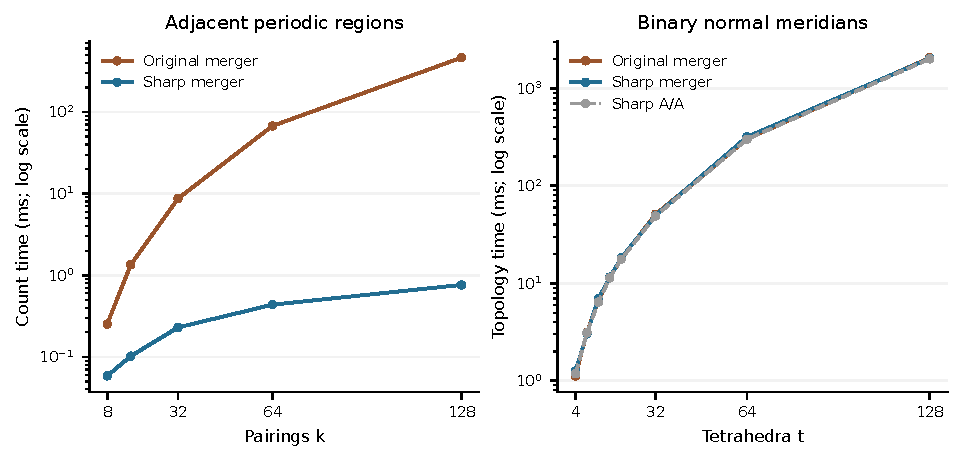
\includegraphics[width=\textwidth]{figures/interval_normal.pdf}
\caption{Measured local queries. Left: the adjacent periodic family with
$p=2^{512}+1$; points join the measured medians and do not represent a
fitted asymptotic law. Right: the complete native topology query for the
layered meridians, including validation and all three orbit counts.
Axes use logarithmic elapsed time. The normal-family curves do not show
a uniform timing advantage for the sharper merger.}
\label{fig:normal}
\end{figure}

The general AHT adapter should not replace the inherited specialized
extreme-ray disc check on the assumption that it will always be faster.
That check can be substantially cheaper on a primitive extreme-ray
meridian. The new adapter answers a broader question: it accepts arbitrary
admissible normal vectors and handles disconnected and one-sided surfaces.
The benchmark also scales a fixed meridian by powers of two through
$2^{2000}$ and verifies the resulting component count exactly. These
large-scale checks are supplementary correctness cases, not a timed
benchmark with repeated samples.

\subsection{Scalar equations on constructed and natural inputs}

Two kinds of valid homogeneous two-term algebraic complexes expose the
coefficient reduction. The sparse family uses two morphism coefficients
and field blocks of degree $d$. At $d=10$ it has 40 objects and 800 original
scalar variables, within the existing default admission cap. Forest
substitution leaves 400 variables. All arms recover the same
20-dimensional full commutant and the same complete compressed complex.
The experiment includes the cost of lifting and canonicalizing the basis.

\begin{table}[htbp]
\centering\small
\setlength{\tabcolsep}{4pt}
\begin{tabular}{@{}rrrrrrr@{}}
\toprule
$d$ & Objects & Direct ms & Span ms & Forest ms & Direct/forest & A/A\\\midrule
4 & 16 & 1.232 & 1.217 & 1.250 & 0.985 & 1.012\\
8 & 32 & 7.423 & 6.051 & 5.553 & 1.305 & 0.957\\
10 & 40 & 12.625 & 10.207 & 9.660 & 1.317 & 1.000\\
\bottomrule
\end{tabular}
\caption{Sparse two-field algebraic family: complete compression-pass medians.}
\label{tab:sparse}
\end{table}


The dense family keeps 16 objects and 128 original variables fixed.
Its two independent homogeneous coefficients partition the degree
$\lfloor b/2\rfloor$ dot monomials according to a chosen variable.
The actual coefficient rank is two, although an ambient coefficientwise
expansion generates thousands of equations. At $b=12$, the equation count
drops from 59\,136 to 128 under span reduction, and to 64 after the forest
substitution. The forest has 64 remaining variables. Table~\ref{tab:dense}
includes the entire compression pass, not merely Gaussian elimination.

\begin{table}[htbp]
\centering\small
\setlength{\tabcolsep}{4pt}
\begin{tabular}{@{}rrrrrrr@{}}
\toprule
$b$ & Direct equations & Span equations & Direct ms & Span ms & Direct/span & A/A\\\midrule
8 & 4480 & 128 & 12.856 & 2.000 & 6.530 & 0.994\\
10 & 16128 & 128 & 60.286 & 4.111 & 14.666 & 0.972\\
12 & 59136 & 128 & 516.973 & 12.815 & 38.521 & 0.996\\
\bottomrule
\end{tabular}
\caption{Dense homogeneous coefficients: equations and complete compression timings. Every row has 128 original variables; the forest has 64 variables and 64 equations.}
\label{tab:dense}
\end{table}


\begin{figure}[htbp]
\centering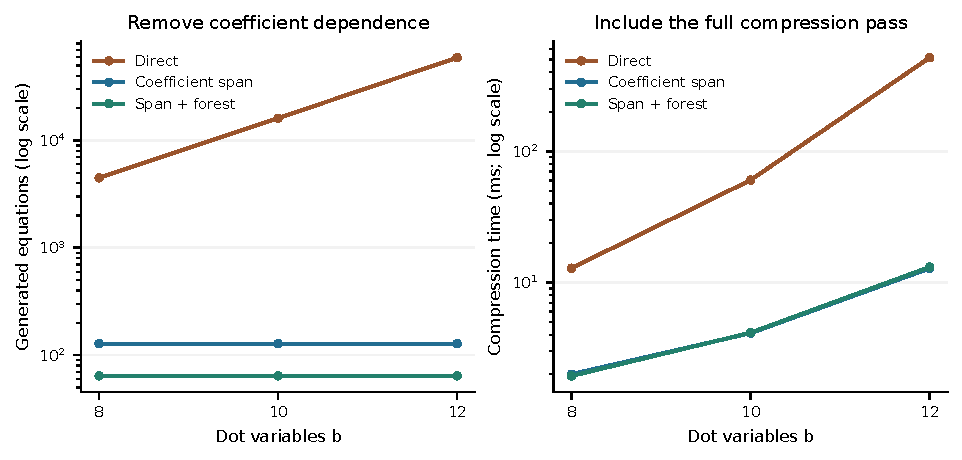
\includegraphics[width=\textwidth]{figures/scalar_coefficients.pdf}
\caption{Constructed homogeneous algebraic family, with no claimed
classical-knot realization. Left: generated scalar equation counts.
Right: complete compression-pass medians, including basis reconstruction.
The ambient coefficient values are still packed binary integers; their
bit length is part of the input and is not treated as constant.}
\label{fig:scalar}
\end{figure}

These are mathematically valid chain-complex examples, checked for
$D^2=0$ and grading consistency. They demonstrate an avoidable ambient
coefficient factor. They do not demonstrate that natural knot prefixes
attain this gap, nor polynomial time in $b$: the packed input itself can
have length exponential in the number of dot variables.

The natural-knot experiment freezes real scalar-solve inputs from three
scans. Summed across their eligible prefix solves, it finds the reductions
in Table~\ref{tab:natural_counts}. ``Remaining variables'' refers to the
reduced equation system; every returned basis is still expressed in the
full original variable space.

\begin{table}[htbp]
\centering\small
\setlength{\tabcolsep}{4pt}
\begin{tabular}{@{}lrrrrrr@{}}
\toprule
Input & Solves & Direct eq. & Span eq. & Forest eq. & $V$ & $V_F$\\\midrule
Conway & 10 & 1310 & 853 & 643 & 590 & 403\\
Kinoshita--Terasaka & 9 & 1324 & 905 & 699 & 551 & 362\\
5-braid stress (36) & 5 & 237 & 194 & 93 & 97 & 35\\
\bottomrule
\end{tabular}
\caption{Actual prefix commutants: sums of per-solve counts, not one simultaneous system.}
\label{tab:natural_counts}
\end{table}


Activation is therefore real. Nevertheless, the complete raw homology
scans in Table~\ref{tab:scans} show no consistent speedup. These scans run
the selected Khovanov backend directly, bypassing earlier recognition
filters so that they actually exercise its scalar machinery. They are
not full recognition-pipeline timings. No ordering search is included
in the timed calls; all arms use the same precomputed order, and their
graded homology agrees with the ordinary exact reference scan.

\begin{table}[htbp]
\centering\small
\setlength{\tabcolsep}{4pt}
\begin{tabular}{@{}lrrrrrr@{}}
\toprule
Input & Direct ms & Span ms & Forest ms & D/span & D/forest & A/A\\\midrule
Conway & 7.917 & 8.294 & 8.864 & 0.959 & 0.851 & 0.970\\
Kinoshita--Terasaka & 8.606 & 9.177 & 9.836 & 0.938 & 0.887 & 1.024\\
Hard unknot (8) & 0.713 & 0.757 & 0.715 & 1.017 & 0.949 & 0.925\\
5-braid stress (36) & 453.776 & 454.439 & 451.814 & 1.000 & 1.055 & 1.059\\
$T(3,5)$ & 3.062 & 3.000 & 2.865 & 1.026 & 1.037 & 1.044\\
\bottomrule
\end{tabular}
\caption{Complete raw homology scans with identical scan order and graded answer. Ratios are median paired ratios. Values near one should be read alongside the A/A control.}
\label{tab:scans}
\end{table}


Transport overhead, small original systems and work elsewhere in the scan
can absorb the reduced solve cost. The maintained default consequently
remains \code{direct}; \code{span} and \code{forest} are explicit options.
A blanket recommendation to enable forest reduction on every prefix
would go beyond these measurements.

\subsection{Whole knot queries and the explicit overlap kernel}

The relator corpus contains twelve maintained survivor unknot diagrams,
two of their mirrors, the 141-crossing Gordian unknot, and four nontrivial
controls. Each is run with the explicit and the compressed group-search
configuration. Four arms compare the historical pairwise query, its A/A
copy, the new adaptive query and the shared index alone. All 760 measured
whole queries, together with 152 excluded warmups, complete with the
expected result. No censored or inconclusive result is silently converted
to a successful timing. Full PD encodings, configurations, status records
and certificate hashes are included in the raw JSON.

\begin{table}[htbp]
\centering\small
\setlength{\tabcolsep}{4pt}
\begin{tabular}{@{}lrrrrrr@{}}
\toprule
Search mode & Pairwise ms & Adaptive ms & Joint ms & P/adaptive & P/joint & A/A\\\midrule
explicit & 830.706 & 490.701 & 931.036 & 1.766 & 0.920 & 1.068\\
compressed & 1357.319 & 1045.271 & 1487.001 & 1.297 & 0.911 & 1.008\\
\bottomrule
\end{tabular}
\caption{Complete configured Gordian recognition queries, including independent replay. The explicit-query replacement can also be reached inside the configured compressed route.}
\label{tab:gordian}
\end{table}


The Gordian improvement is attributable to one residual overlap query,
after 129 generator eliminations. It has twelve nonempty relators of
total length 17\,504. The maximum guaranteed gain is 2\,998, and the
adaptive prelude needs four oriented donor automata in place of 24.
The selected move and the complete 141-move certificate are unchanged on
this input. The independent replay modules do not use the producer's
shared index. Tests also disable producer-only helpers during replay,
so accepting the optimized search output is not circular.

The shared index by itself regresses on Gordian. This negative arm is
retained in the table. Its larger construction cost is justified for
many relators, whereas Gordian admits strong incumbent bounds early.
The fixed four-relator base case avoids paying a failed prelude followed
by shared construction on very small lists. The initial measurement run,
which motivated that base case, is retained separately as calibration
data together with the matching index source; it is not mixed into the
final medians.

\begin{table}[htbp]
\centering\small
\setlength{\tabcolsep}{4pt}
\begin{tabular}{@{}lrrrrrr@{}}
\toprule
Input & $\ell$ & Gain & Pairwise ms & Adaptive ms & Joint ms & P/adaptive\\\midrule
Gordian residual & 17504 & 2998 & 265.052 & 62.032 & 416.868 & 4.232\\
$8\times64$ random & 512 & 0 & 8.249 & 9.809 & 7.025 & 0.859\\
$32\times64$ random & 2048 & 0 & 129.521 & 46.800 & 26.003 & 2.768\\
$128\times64$ random & 8192 & 0 & 2066.899 & 231.601 & 185.595 & 8.798\\
Periodic duplicates & 32768 & 1024 & 74.049 & 4.485 & 311.439 & 16.510\\
\bottomrule
\end{tabular}
\caption{Exact explicit overlap queries, including all index construction and any failed prelude. Only the first row comes from the measured knot presentation; the others are synthetic capacity cases.}
\label{tab:overlap_kernels}
\end{table}


The random relator rows are exact-query capacity experiments, not knot
recognition results. Their optimum gain is zero, so a correct query must
rule out every eligible shortening. On the 128-by-64 case the simultaneous
index removes the repeated target scans, and the adaptive route retains
most of the benefit even after charging its failed prelude. The eight-by-64
case is a counterexample to universal practical improvement: the adaptive
query can be slower. Highly repetitive duplicate relators favor early
donor bounds, again making the adaptive route preferable to always
building the shared index. No single timing arm is best on every row.

\subsection{Independent correctness and validation coverage}

The mathematical specifications are checked by several different oracles.
The interval suite compares both merger policies with literal disjoint-set
connectivity on 9\,882 small two-pairing systems, exhaustive tiny triples
and 2\,000 randomized systems. It exhausts the relevant two-period
thresholds for periods through twelve, checks invalid endpoints and
shared budgets, and includes 700 independently counted signed systems.
Large integer tests ensure that bit length, rather than represented
interval size, determines storage.

The normal-surface suite checks explicit arc graphs, reoriented and
relabelled triangulations, the zero surface, vertex-linking discs,
essential meridians and one-sided M\"obius families. It compares normal
surfaces and compatible sums in small layered triangulations against
Regina 7.4 for connected components, orientability, boundary count, Euler
characteristic and compressing-disc status \cite{regina}. It also compares
the native ambient validator against Regina on the enumerated one-face
gluing cases. Regina is an optional independent test dependency; neither
new production module imports it.

The scalar suite reconstructs coefficient entries, exhausts 256 small
two-coefficient matrix systems, checks randomized rectangular blocks and
compares the canonical complete nullspace in all modes. It verifies
actual split witnesses, static child-commutant reuse and the existing
admission caps. These tests establish equality of the object used by the
bounded candidate policy, not just equality of nullity.

The overlap suite checks 7\,056 exhaustive small ordered word pairs,
350 small multisets against a literal all-rotation oracle, and 600 larger
multisets against the historical query. Cases include inverse donors,
periodic words, zero-length slots, equal words in distinct slots, cap
boundaries, cancellation, malformed witnesses and tampered certificates.
The exhaustive and differential comparisons require the same optimal
gain and a valid attaining witness; the general shared index is allowed
to choose a different tied witness. Complete corpus certificates are
also compared explicitly.

\paragraph{Full integration gate.}
With the pinned sibling reference dependencies restored, the untouched
baseline runs 768 test methods: 767 pass and one fails with the inherited
delayed-input subprocess timeout. The maintained overlay passes all
\textbf{807 test methods}, with no failures, errors or skips. The integrated
run includes the repaired worker regression and 39 additional test methods;
many methods contain large exhaustive or randomized families. The baseline
and maintained runs report 112.659 and 120.692 seconds respectively. These
different-size suite durations are validation records, not a performance
comparison. Source hashes are unchanged throughout both runs, and the
446-file baseline staging archive remains byte-identical. Full logs and a
machine-readable summary accompany the article.


\section{Integration contracts and implementation decisions}
\label{sec:integration}

The archive supplies an overlay at the original repository-relative paths
and a binary-capable Git patch against the pinned baseline. The patch is
verified by applying it to a clean reconstruction of the affected baseline
files and comparing the resulting bytes with the overlay. It includes the
article and reproducibility artifacts; no remote branch or publication is
created as part of this delivery.

\subsection{Production and research interfaces}

The exact interval kernel is a standalone native Python module. A minimal
query, run with \path{fast/} on the import path, is:

\noindent\begin{minipage}{\linewidth}
\begin{lstlisting}[language=Python]
from fastunknot.interval_orbits import IntervalPairing, count_orbits

p = 2**512 + 1
pairs = [IntervalPairing(i*p, (i+1)*p-1,
                         (i+1)*p, (i+2)*p-1)
         for i in range(128)]
answer = count_orbits(129*p, pairs, max_cycles=1000)
assert answer.complete and answer.orbits == p
\end{lstlisting}
\end{minipage}

Endpoints are inclusive and zero-based. A pairing must have equal domain
and range widths. \code{periodic\_rule="aht"} selects the original merger
for comparison; the default is \code{"fine\_wilf"}. Signed counting and
point-membership queries reuse the same exact kernel. A cycle limit is
shared across the constituent counts. An exhausted query returns an
incomplete result, and a caller-provided cancellation callback propagates
its exception. Neither condition is interpreted as a negative theorem.

The normal-surface adapter can be exercised on a supplied layered meridian:

\noindent\begin{minipage}{\linewidth}
\begin{lstlisting}[language=Python]
from normal_orbit_research.fixtures import layered_torus
from fastunknot.normal_surface_orbits import normal_surface_topology

triangulation, coordinates = layered_torus(32)
topology = normal_surface_topology(
    triangulation, coordinates, max_cycles=10000)
assert topology['status'] == 'COMPLETE'
assert topology['components'] == 1
assert topology['compressing_disk']
\end{lstlisting}
\end{minipage}

This result concerns the provided triangulation. It is not a top-level
recognition verdict. The inherited constructor is included for research
and tests, with provenance pointing to report 36; the production adapter
does not depend on that constructor.

The scalar options are deliberately explicit:

\noindent\begin{minipage}{\linewidth}
\begin{lstlisting}[language=Python]
from fastunknot.scalar_split import fitting_khovanov_rank

answer = fitting_khovanov_rank(
    pd, fitting_primary=True, fitting_coefficient_mode='forest')
# Other modes: 'direct' (the maintained default), 'span'.
\end{lstlisting}
\end{minipage}

The lower-level scalar-space and scalar-split functions likewise accept
\code{coefficient\_mode}. The full original basis is returned in every
mode. New counters expose coefficient rank, equation counts, forest
edges, original variables and reduced variables. Existing admission caps,
type distinctions, witness checks and cache-invalidation rules are
preserved.

The explicit overlap entry point now defaults to \code{backend="adaptive"}.
The optional values \code{"pairwise"} and \code{"joint"} isolate the
incumbent and shared-index strategies for audits. This change applies when
an existing configured group search calls the explicit overlap query; it
does not automatically enable an otherwise disabled group stage or remove
an explicit expansion cap. The existing certificate fields and independent
replayers remain unchanged.

\subsection{Two correctness repairs exposed by the audit}

The public scalar-space shortcut for an all-singleton closed group formerly
returned only the common identity. For a disconnected declared group, the
correct space contains one component-indicator scalar for each weak
component. The empty group similarly has a zero-dimensional endomorphism
space, rather than a basis list containing the zero vector. The shortcut
now handles these cases and rejects malformed duplicate or nonclosed
groups. Internal connected scanner calls retain their prior mathematical
behavior. These statements concern the declared scalar partition; the
change does not recover unknown relative quantum shifts between unrelated
components.

The maintained normal-surface subprocess wrapper also had a reproducible
partial-input deadlock in this CPython environment. Its polling loop sent
the payload in the first \code{communicate} call and retried with no input
after a timeout. If the child delayed reading a large payload, later polls
could leave the unsent remainder pending indefinitely. The existing
regression test exposed this failure in the untouched baseline.

The repair stages UTF-8 input and captures output in private temporary
standard streams, then polls the child's public \code{wait} interface.
This avoids repeated partial pipe communication. Cancellation and deadline
checks cover preparation, waiting and output collection; exceptional exits
kill and reap the child and close the streams. The tests retain strict
cleanup checks and add Unicode plus large-output coverage. This is a
correctness repair, with a temporary-storage tradeoff, and is not included
in the reported quotient-kernel speedups.

\subsection{Claims at the integration boundary}

\begin{center}\small
\begin{tabularx}{\textwidth}{@{}p{33mm}XX@{}}
\toprule
Component & Established here & Remaining boundary\\\midrule
Interval orbits & Exact counts; sharper merger; polynomial encoded query & Weighted component data and attachment extraction\\
Normal topology & Native validation and topology for an admissible supplied vector & Surface search, cut output and knot-exterior correspondence\\
Scalar solve & Same full canonical commutant with fewer equations or unknowns & Uniform bounds on multiplicities, coefficient encoding and reconstruction\\
Cyclic overlap & Exact maximum guaranteed shortening with a near-linear local query & Total presentation growth, successful move count and completeness\\
Complete pipeline & Passing integration tests and measured Gordian improvement & A general quasi-polynomial worst-case proof\\
\bottomrule
\end{tabularx}
\end{center}

The integration favors explicit contracts: each reusable local operation
states its input representation, its resource behavior, and what its
answer certifies. This makes later research failures informative. For
example, if a compressed cutting implementation needs information absent
from an orbit-count result, it must extend that result's contract rather
than quietly reconstruct an exponentially large surface.

\section{Sufficient global bounds and a concrete research agenda}
\label{sec:global-agenda}

The local theorems expose several quantities that could support a global
bound. At present these quantities describe an execution; they are not
proved restrictions on every diagram. The next task is to convert selected
observations into uniform bounds, while retaining an algorithm that always
finishes with a correct decision.

\subsection{A sufficient accounting principle}

Let $S_*(n)$ bound the complete bit length of every state, query input,
output, and retained certificate record in an execution. Let $Q_*(n)$ bound
the number of charged operations, including failed branches, hierarchy
repairs, canonicalization, certificate verification and changes of
representation. Fixed constants in local polynomial algorithms must be
uniform over the allowed input family. In particular, a handle-type catalog
or a frontier alphabet whose size grows with $n$ cannot be hidden inside
such a constant.

\begin{proposition}[Conditional composition bound]
\label{prop:global-accounting}
Suppose a sound and complete recognition algorithm has preprocessing time
$P(n)$, makes at most $Q_*(n)$ calls, and each call costs at most
$C(1+S_*(n))^a$ bit operations for fixed $C,a$. If, for fixed
$\alpha,\beta,\gamma\ge1$,
\[
\begin{split}
 Q_*(n)&\le\exp(O(\log^{\alpha}(n+2))),\\
 S_*(n)&\le\exp(O(\log^{\beta}(n+2))),\\
 P(n)&\le\exp(O(\log^{\gamma}(n+2))),
\end{split}
\]
then its total time is
$\exp(O(\log^{\max(\alpha,\beta,\gamma)}(n+2)))$.
In particular, exponents at most two suffice for $n^{O(\log n)}$.
\end{proposition}

\begin{proof}
The total time is at most $P(n)+C Q_*(n)(1+S_*(n))^a$.
Taking logarithms of the second term adds the bounds for $\log Q_*$
and $a\log(1+S_*)$. A fixed finite sum of these logarithmic powers is
bounded by a constant times the largest one. Adding preprocessing does
not change that largest exponent.
\end{proof}

The proposition is an accounting criterion, not a theorem that its
hypotheses hold for the present recognizer. Polynomial time for a local
query does not bound $Q_*$ or $S_*$. An inconclusive budget exit does not
supply completeness. Nor does a short successful certificate show that a
deterministic search finds it within the same bound. All expanded data
that must actually be written count towards the relevant size and time.

\subsection{Hierarchy depth, restarts and branching are separate parameters}

Write $H$ for maximum hierarchy length and $G$ for maximum pattern
complexity. In this notation Lackenby's Proposition~9.1 gives the iteration
bound $H(G+1)^H$ \cite{lackenby2026}. Hence a sufficient restriction for
this part of the calculation is
\[
                 H\log(G+1)+\log(H+1)=O(\log^2 n).
\]
For example, $H=O(\log n)$ and $G=n^{O(1)}$ suffice. If instead
$H=O(\log^2 n)$ and $G=n^{O(1)}$, this particular bound gives
$\exp(O(\log^3 n))$: quasi-polynomial in the broader sense, but not the
specific $n^{O(\log n)}$ target. A polynomial bound on the bit length of
$G$ alone does not imply $G=n^{O(1)}$.

The refined construction in Section~10 controls hierarchy length linearly
in the initial $q$-complexity. It does not by itself give logarithmic
depth or a quasi-polynomial bound on the restart expression. Conversely,
replacing a costly surface-topology query by AHT lowers the cost of one
step without lowering the number of lexicographic repairs. These are
different improvements and require different proofs.

If a proposed construction has at most $B(n)$ possible children at depth
at most $H(n)$, its search tree can contain as many as
$\sum_{j=0}^{H(n)}B(n)^j$ nodes. Polynomial branching and logarithmic
depth are sufficient for a quasi-polynomial tree-size bound. Polynomial
depth is not. Revisiting or modifying a node requires an additional
amortized bound, even if the number of distinct nodes is controlled.
Memoization helps only after proving that the canonical state retains
every relevant boundary marking and that the number of such states is
small. A state with polynomially many bits can still have exponentially
many possible values.

\paragraph{Falsifiable hierarchy question.}
For the multisurface and generalized-Heegaard construction, identify a
potential that pays both for ordinary progress and for discarding later
surfaces after a repair. Can every long execution produce a certified
Cheeger-region simplification before the restart cost exceeds a
polylogarithmic exponent? Useful negative instances would keep the
recorded local complexities small while forcing many successive repairs.
Such examples would refute a proposed potential, even if all topology
queries themselves were fast. The announced acceleration framework
\cite{lackenbytalk} motivates this question; the present kernels do not
implement its global argument.

\subsection{From normal-coordinate topology to certified cutting}

The current normal adapter supplies connectivity and total topological
statistics for a supplied surface. A compressed cutting primitive has a
larger contract. It must return the complementary handle structure,
the parallelity components, the topology and twisting of their base
surfaces, and the attachment of their vertical boundaries. These are the
kinds of output required by Lackenby's Theorem~14.4
\cite{lackenby2026}. Matching component counts do not determine these
attachments. Even matching unmarked surface types does not determine a
map relative to a marked boundary.

The first implementation target is weighted AHT with grouped multiplicity
records, followed by a compiler from those records to the required cut
incidence data. The weighted orbit theorem is classical \cite{aht}; its
implementation would extend the current module rather than establish a
new existence theorem. Its output must remain grouped when a binary vector
describes exponentially many equal components. Explicitly listing one
record per component defeats the compression.

A useful contract for testing is a commuting reconstruction diagram:
on small inputs, expand the original surface and perform an independent
ordinary cut; expand the compressed output; compare the resulting marked
cell structures. Include twisted bundles, annular interfaces,
self-identifications, boundary-parallel discs and disconnected surfaces.
For large inputs, retain locally checkable construction records instead
of treating a numerical topology summary as a reconstruction proof.

An equally important target is a verified diagram-to-exterior adapter.
It must specify how the peripheral torus corresponds to the knot and how
that correspondence changes during simplification. A normal disc whose
boundary is essential in a supplied torus certifies compression of that
torus. Turning it into a certificate about the input PD diagram requires
the exterior correspondence. A complete global theorem also needs a
method of finding suitable surfaces within its work budget.

\subsection{Frontier and representation bounds}

Let $w$ be the number of interface positions in a scanner state, $\tau$
the number of retained scalar types, $\mu=\max_v s_v$, $E$ the number of
nonzero typed blocks, $\rho=\max_{u,v}\rho_{uv}$, and $B$ the largest
packed morphism bit length. The elementary inequalities
\[
              V\le\tau\mu^2,\qquad
              P_{\mathrm{span}}\le E\rho\mu^2
\]
describe how these parameters enter the solver. They do not bound the
parameters in terms of $n$. A small coefficient span does not bound
multiplicity, and small frontier width does not by itself bound the
size of all coefficients or the number of repeated states.

One sufficient approach is to prove a uniform encoding bound of the form
$S_*\le\exp(O(w\log(w+2)))\poly(n)$ and a suitable bound on all visits,
then establish $w\log(w+2)=O(\log^2 n)$ for the chosen decomposition or
for an exact quotient of its states. This is a proposed route, not a
property established for the present scanner. A square-root-width
separator bound, even if available for a particular diagram graph, would
give a much larger exponent in this model and would not meet the target.

The experiment should record $w,\tau,\mu,E,\rho,B,V,V_F$, reconstruction
cost, and the number of repeated states together. Search for families in
which one proposed controlling parameter stays fixed while another grows.
In particular, a useful challenge to the forest proposal is a family with
small $V_F$ but costly dense reconstruction in the original $V$ variables.
The current bounded-candidate policy requires that reconstruction, so it
cannot be excluded from the accounting.

\subsection{A tractable commutant family and its limitations}

There is a clean special case in which the forest construction supplies
explicit projections, rather than merely a smaller linear system.

\begin{proposition}[Scalar transports give explicit repeated summands]
\label{prop:scalar-transport-splitting}
Consider an entire finite differential component with no incident
differential blocks omitted. Suppose every scalar type has multiplicity
$s$ and the selected invertible forest connects all its types. Use the
transport matrices $P_v$ from Theorem~\ref{thm:forest}. The complete
commutant is the common centralizer in $M_s(\F)$ of every transported
coefficient matrix $P_v^{-1}A_iP_u$.

If every such matrix is a scalar multiple of $I_s$, the component is
isomorphic to a direct sum of $s$ identical multiplicity-one typed
complexes. Explicit compatible matrix units in the original coordinates
are
\[
                   E^{(v)}_{ij}=P_v E_{ij}P_v^{-1}.
\]
In particular, the $s$ diagonal units are orthogonal rank-one projectors
whose sum is the identity. If additional attachment maps are required in
the splitting contract, the assertion applies when they also respect
these summands; this must be verified, not inferred from the differential.
\end{proposition}

\begin{proof}
There is one root matrix $X$ because the forest is connected. Theorem
\ref{thm:forest} changes every original equation into $X\widetilde A_i
=\widetilde A_iX$, proving the centralizer statement. Under the scalar
hypothesis every $X\in M_s(\F)$ satisfies these equations. After changing
the basis at type $v$ by $P_v$, each differential block is a morphism
coefficient times $I_s$, since all of its scalar coefficient matrices
are scalar. The $s$ coordinate lines are therefore invariant and carry
identical typed differentials. Conjugating the usual matrix units back
gives the displayed formula, their multiplication identities, and the
rank-one projections. Their images supply the claimed direct sum. The
same conclusion for extra attachments follows only if the required
invariance or transported block form is checked for those maps as well.
\end{proof}

A sufficient case is that the graph of all nonzero typed blocks is a
tree and each block has a one-dimensional coefficient span whose nonzero
coefficient matrix is invertible. Choosing those matrices as the forest
transports turns every block coefficient matrix into $I_s$. This is an
algebraic family; its prevalence among actual knot-scan components remains
an empirical and structural question. The current implementation computes
and canonically reconstructs the full commutant. It does not yet bypass
the bounded candidate policy with these direct projectors.

Cycles explain a limitation. A non-tree invertible block becomes a
holonomy constraint on $X$, and all noninvertible coefficients impose
their own centralizer conditions. If these matrices have only the scalar
common centralizer, there are no nontrivial projections in that algebra.
Thus a connected invertible forest does not guarantee a useful split.
At the other extreme, low-rank coefficient spans need not display an
invertible basis element: the two singular matrices
$\operatorname{diag}(1,0)$ and $\operatorname{diag}(0,1)$ span $I_2$.
The current forest search can therefore miss an invertible linear
combination. Exhausting the span costs $2^\rho$ candidates, so any wider
search needs a stated rank restriction or its own complexity argument.

\subsection{Explicit and compressed relator growth}

The new shared query costs nearly linearly in the total explicit relator
length $\ell$, with the stated logarithmic and dictionary-model factors.
Its speed does not make $\ell$ small. Generator substitution can duplicate
long words across many relators; a sequence of individually valid moves
can therefore create an expensive explicit presentation before the next
shortening query is reached.

There is a modest unconditional observation for a restricted phase: if
every accepted relator replacement strictly decreases total explicit
length, and no intervening operation increases it, the number of such
replacements is at most the starting length. This says nothing about
whether that phase recognizes every unknot, and it does not bound the
length at entry to later phases. A useful next theorem would control
both presentation growth and the number of verified moves across the
whole producer, including generator eliminations and Whitehead steps.

For straight-line representations, track grammar size, logarithmic
represented length, the number of rewritten nonterminals, and the cost
of checking each move. A shared fully compressed cyclic index would
need to handle donor exclusion and occurrence deletion without expanding
the rotations. An incremental explicit index is another concrete target,
but reusing an index after mutation requires exact removal of obsolete
occurrences. Each proposal should be challenged by presentations where
short descriptions expand rapidly or where most indexed occurrences are
invalidated by a single certified move.

\subsection{Proposed research questions}

The following questions are prioritized by how directly they remove a
known implementation or proof obstruction. They can be pursued separately,
but every claimed global application must satisfy the complete accounting
contract above.

\begin{enumerate}[label=Q\arabic*.,leftmargin=12mm]
\item \textbf{Weighted component extraction.} Can the native interval
kernel return selected component coordinates and grouped topological
weights in polynomial encoded time, including one-sided components and
exponentially large multiplicities?
\item \textbf{Marked cutting.} What is the smallest attachment record that
determines the cut complement and its parallelity bundles relative to all
peripheral markings? Can its expansion be independently compared with
ordinary cutting on every small test input?
\item \textbf{Exterior correspondence.} Can each diagram simplification and
exterior construction emit a short composable certificate preserving the
peripheral identification needed by the final compressing-disc argument?
\item \textbf{Hierarchy repairs.} Is there an amortized potential that bounds
the cumulative cost of discarded and rebuilt hierarchy suffixes by
$\exp(O(\log^2 n))$, or an explicit family refuting a proposed potential?
\item \textbf{Interface compression.} Which exact state equivalence can
reduce the effective interface description below the width of the raw
diagram decomposition while preserving every future attachment operation?
\item \textbf{Natural coefficient ranks.} Are there topologically defined
knot families with uniformly small $\rho_{uv}$ but growing ambient
coefficient support, and can the rank advantage persist after including
all scan and reconstruction costs?
\item \textbf{Constructive scalar summands.} Can the transported-projector
family of Proposition~\ref{prop:scalar-transport-splitting} be recognized
and split directly under the scanner's full attachment contract, avoiding
construction of its entire commutant basis?
\item \textbf{Invertible combinations.} For the coefficient spaces actually
arising in the scanner, can an invertible linear combination be found with
a proved cost smaller than enumerating all $2^\rho$ combinations?
\item \textbf{Canonical output cost.} Can candidate selection be reformulated
in reduced root coordinates with an independently verified equivalence to
the existing policy, so that a large full-basis reconstruction is avoided?
\item \textbf{Shared compressed word search.} Can capped cyclic windows and
distinct-slot donor constraints be indexed in time polynomial in grammar
size and logarithmic represented length, without expanding the rotations?
\item \textbf{Presentation growth.} For which nontrivial diagram families
are both intermediate presentation size and the full verified move count
quasi-polynomially bounded, including the substitutions that increase
length between shortening phases?
\item \textbf{Incremental exact indices.} Can relator replacement and deletion
update the shared index faster than rebuilding it while deleting every
obsolete occurrence and retaining a compact independently checkable match?
\end{enumerate}

\subsection{Milestones that would justify stronger conclusions}

The next report should distinguish the following outcomes.
\begin{enumerate}
\item A completed weighted-orbit and marked-cutting implementation, with
independent reconstruction tests and a proved bound on its encoded output.
\item A verified connection from the ordinary knot diagram to the
triangulation and peripheral data consumed by the geometric kernels.
\item A structural theorem for a nontrivial diagram family controlling
every parameter in Proposition~\ref{prop:global-accounting}, rather than
only the frontier width or a successful witness size.
\item A constructive implementation of Proposition
\ref{prop:scalar-transport-splitting}, checked against the maintained
attachment contract and measured on actual differential components.
\item A complete presentation-growth and move-count bound for a specified
group-simplification family, or an exact compressed replacement for the
steps that defeat such a bound.
\item A hierarchy theorem paying simultaneously for depth, branching,
repairs and representation changes, with every local oracle instantiated.
\end{enumerate}

Any one of these would close a clearly identified gap. A general
$n^{O(\log n)}$ conclusion requires enough of them, or an alternative
complete route, to meet a uniform total-work bound on every input.


\appendix
\section{Reproducing the numerical report}

From the repository root, first verify and apply \path{integration.patch}
against the pinned baseline. Detailed commands and a checksum manifest
are included in the archive's README. The ordinary full-suite command is
run from \path{Topology/UnknotRecognition/fast}:

\noindent\begin{minipage}{\linewidth}
\begin{lstlisting}[language=bash]
PYTHONPATH=. python3 -B -m unittest discover -s tests -v
\end{lstlisting}
\end{minipage}

The maintained suite has sibling reference dependencies in
\path{reports/24/reference}, \path{reports/26/detshadow} and
\path{reports/28/src/closure_reset}. They must be present at the pinned
commit. A sparse checkout of \path{fast/} alone is insufficient for this
full gate. The independent Regina comparisons are optional tests, but
they were available and ran in the reported environment.

The four experiment entry points, run from \path{fast/}, are:

\noindent\begin{minipage}{\linewidth}
\begin{lstlisting}[language=bash]
python3 -B interval_research/benchmark.py \
  --output interval_research/results.json
python3 -B normal_orbit_research/benchmark.py \
  --output normal_orbit_research/results.json
python3 -B benchmark_coefficient_span.py \
  --output coefficient_research/results.json
python3 -B cyclic_overlap_research/benchmark.py \
  --output cyclic_overlap_research/results.json
python3 -B cyclic_overlap_research/make_summary.py
\end{lstlisting}
\end{minipage}

Use new output paths to retain the shipped samples unchanged. The
benchmark scripts record exact answers and reject disagreements before
producing a successful report. The interval, coefficient and relator benchmarks also check that
their measured source files did not change during the run. The normal
series records end-of-run source hashes; the final static audit checks
all recorded hashes against the supplied files. Random seeds,
warmup policy, repeat counts and source digests are stored in the JSON.

To regenerate the figures and tables, run \path{render_results.py} from
the article directory; it reads the four archived result files at their
repository-relative locations. Matplotlib is required only for this step.
The supplied figure PDFs and tables allow the article to be built without
rerunning any experiment:

\noindent\begin{minipage}{\linewidth}
\begin{lstlisting}[language=bash]
latexmk -pdf -interaction=nonstopmode -halt-on-error article.tex
\end{lstlisting}
\end{minipage}

\section{The complete whole-query corpus}

Table~\ref{tab:corpus} provides the per-input full-query medians in addition
to the focused Gordian comparison. Inputs that never reach the optimized
query are necessary controls. Their nearly identical timings should not
be interpreted as evidence for, or against, the local index theorem.
Every measured run and excluded warmup is retained in the raw corpus.

\begin{table}[htbp]
\centering\small
\setlength{\tabcolsep}{4pt}
\begin{tabular}{@{}lrrrrrrr@{}}
\toprule
Case & $n$ & E pair ms & E adapt ms & E ratio & C pair ms & C adapt ms & C ratio\\\midrule
survivor-00 & 16 & 3.153 & 3.186 & 0.954 & 11.808 & 12.613 & 0.929\\
survivor-01 & 15 & 2.398 & 2.384 & 1.033 & 10.594 & 9.966 & 1.082\\
survivor-02 & 15 & 2.866 & 2.940 & 0.960 & 13.820 & 13.876 & 0.942\\
survivor-03 & 13 & 2.168 & 2.406 & 0.969 & 8.431 & 9.904 & 0.906\\
mirror-03 & 13 & 4.945 & 4.580 & 1.057 & 16.982 & 16.328 & 0.999\\
survivor-04 & 13 & 1.774 & 1.694 & 1.045 & 7.898 & 7.900 & 0.996\\
survivor-05 & 13 & 3.078 & 3.115 & 0.971 & 13.460 & 12.339 & 1.081\\
survivor-06 & 12 & 2.288 & 2.127 & 1.035 & 6.986 & 6.999 & 1.006\\
survivor-07 & 12 & 3.058 & 3.063 & 1.010 & 13.952 & 15.293 & 0.838\\
survivor-08 & 11 & 1.318 & 1.414 & 0.992 & 5.224 & 5.567 & 0.941\\
mirror-08 & 11 & 4.584 & 3.933 & 1.126 & 13.204 & 12.957 & 1.010\\
survivor-09 & 11 & 1.512 & 1.436 & 1.053 & 5.317 & 5.305 & 0.977\\
survivor-10 & 11 & 1.313 & 1.404 & 0.945 & 4.759 & 5.039 & 0.964\\
survivor-11 & 11 & 1.534 & 1.716 & 0.928 & 6.225 & 6.378 & 0.997\\
gordian & 141 & 830.706 & 490.701 & 1.766 & 1357.319 & 1045.271 & 1.297\\
trefoil & 3 & 0.030 & 0.031 & 0.996 & 0.029 & 0.028 & 1.009\\
figure\_eight & 4 & 0.032 & 0.032 & 1.016 & 0.030 & 0.030 & 0.988\\
conway & 11 & 0.609 & 0.593 & 1.085 & 0.659 & 0.669 & 1.028\\
kinoshita\_terasaka & 11 & 0.626 & 0.664 & 0.930 & 0.627 & 0.653 & 0.960\\
\bottomrule
\end{tabular}
\caption{All whole-query cases. E and C denote the explicit and compressed configurations. All statuses are complete and agree with the listed corpus expectations in the raw data.}
\label{tab:corpus}
\end{table}


\section{Attribution and artifact provenance}

The maintained pipeline and layered-torus fixtures belong to the ProveIt
baseline \cite{repository}. The native orbit implementation was written
independently from the AHT paper; no third-party GPL orbit implementation
was imported or copied. The stronger threshold uses Fine--Wilf periodicity
\cite{finewilf}; the graph interpretation has a substantial existing
literature, including Rankin \cite{rankin}. The normal connectivity
reduction and weighted-orbit existence theorem are classical AHT results.
Suffix automata are classical \cite{blumer}, and the coefficient and forest
identities are elementary linear algebra applied to the maintained typed
solver. Bar-Natan's local and formal-complex methods provide the relevant
Khovanov computational setting \cite{barnatan,barnatancob}.

The new package claims these particular implementations, integration
decisions, proofs of their contracts and reproducible observations. It
does not claim priority for the general mathematical ingredients. The
normal validator is adapted from report 36's native certificate checker;
the inherited fixture file is identified separately in the provenance
record. Regina is used only as an external independent test oracle and is
not redistributed as production source in this archive.

\begin{thebibliography}{99}
\raggedright
\bibitem{repository}
V. Reshetnikov, \emph{ProveIt: Topology/UnknotRecognition},
pinned commit \texttt{58ee11a97d5fd7f21647c57eefaf3ecc007931d6},
8 October 2026.
\url{https://github.com/VladimirReshetnikov/ProveIt/tree/58ee11a97d5fd7f21647c57eefaf3ecc007931d6/Topology/UnknotRecognition}.

\bibitem{lackenby2026}
M. Lackenby, \emph{Incompressible surfaces, hierarchies and unknot
recognition}, arXiv:2607.23350v1, 25 July 2026.
\url{https://arxiv.org/abs/2607.23350}.
Sections 9--10 are especially relevant to iteration and hierarchy-length
bounds. No general running-time estimate is imported from these statements.

\bibitem{lackenbytalk}
M. Lackenby, \emph{Unknot recognition in quasi-polynomial time},
lecture slides, 2021.
\url{https://people.maths.ox.ac.uk/lackenby/quasipolynomial-talk.pdf}.

\bibitem{aht}
I. Agol, J. Hass and W. P. Thurston,
\emph{The computational complexity of knot genus and spanning area},
Transactions of the American Mathematical Society \textbf{358} (2006),
3821--3850. Preprint arXiv:math/0205057.
\url{https://arxiv.org/abs/math/0205057}.
The unweighted orbit algorithm is in Section 4, Theorem 12;
normal-surface connectivity is Corollary 14; weighted orbit data are
treated in Section 6.

\bibitem{finewilf}
N. J. Fine and H. S. Wilf, \emph{Uniqueness theorems for periodic
functions}, Proceedings of the American Mathematical Society
\textbf{16} (1965), 109--114.
\url{https://doi.org/10.1090/S0002-9939-1965-0174934-9}.

\bibitem{rankin}
S. A. Rankin, \emph{Fine--Wilf graphs and the generalized Fine--Wilf
theorem}, arXiv:0906.1780, 2009.
\url{https://arxiv.org/abs/0906.1780}.
This gives a primary research treatment of the graph viewpoint on
periodicity.

\bibitem{blumer}
A. Blumer, J. Blumer, D. Haussler, A. Ehrenfeucht, M. T. Chen and
J. Seiferas, \emph{The smallest automaton recognizing the subwords
of a text}, Theoretical Computer Science \textbf{40} (1985), 31--55.
\url{https://doi.org/10.1016/0304-3975(85)90157-4}.

\bibitem{barnatan}
D. Bar-Natan, \emph{Fast Khovanov homology computations},
Journal of Knot Theory and Its Ramifications \textbf{16} (2007),
243--255. \url{https://arxiv.org/abs/math/0606318}.

\bibitem{barnatancob}
D. Bar-Natan, \emph{Khovanov's homology for tangles and cobordisms},
Geometry and Topology \textbf{9} (2005), 1443--1499.
\url{https://arxiv.org/abs/math/0410495}.

\bibitem{regina}
The Regina development team, \emph{Regina calculation engine:
NormalSurface reference}, official documentation.
\url{https://regina-normal.github.io/engine-docs/classregina_1_1NormalSurface.html}.
The local independent checks in this package used Regina 7.4;
the native production orbit and normal-coordinate modules do not
import Regina.
\end{thebibliography}

\end{document}
